\documentclass[11pt]{article}
\usepackage[T1]{fontenc}
\usepackage{lmodern}
\usepackage[margin=1in,letterpaper]{geometry}
\usepackage{amsmath,amssymb,booktabs,array,xcolor}
\usepackage{textcomp}
\usepackage[hidelinks]{hyperref}
\usepackage{graphicx}
\graphicspath{{paper_figures/}{./}{../paper_figures/}}
\usepackage{tabularx}
\usepackage{caption}
\captionsetup{font=small,labelfont=bf,skip=4pt}
\usepackage{placeins}
\usepackage{float}
\renewcommand{\topfraction}{0.9}
\renewcommand{\bottomfraction}{0.85}
\renewcommand{\textfraction}{0.07}
\renewcommand{\floatpagefraction}{0.75}
\setcounter{topnumber}{4}
\setcounter{bottomnumber}{4}
\setcounter{totalnumber}{8}
\emergencystretch=2.5em

\newcommand{\eebar}{\bar{e}_{31}}
\newcommand{\Xibar}{\bar{\Xi}_{33}}

\title{\bfseries Exact Radial-Determinant Frequencies of a Piezoelectric
Annular Plate, and Inverse Recovery of $e_{31}$ from Open-Circuit Flexure}
\author{Garrek McCune$^{a,*}$, Daniel Stutts$^{a}$\\
\small\itshape $^a$Mechanical and Aerospace Engineering,\\
Missouri University of Science and Technology, Rolla, MO 65409, USA\\
\small\upshape $^*$Corresponding author. E-mail: ghmkfh@umsystem.edu}
\date{DRAFT --- \today}
% Supplementary Material mapping (PAPER4_PIEZO_SUPPLEMENTARY.tex):
%   S.1  cubic consistency condition and open-circuit rank-1 coefficient
%   S.2  inverse G2 cross-checks
%   S.3  F-F FE discriminator and mixed-BC outer-only ground
%   S.4  wide-axis admittance figure
%   S.5  thickness-ratio sweep and Y at 1/8, 1/5
%   S.6  cluster job provenance
%   S.7  mixed-edge C-F / F-C closed form
% Main text contains no job numbers.

\begin{document}
\maketitle

\begin{abstract}
A steel annular plate with identical thickness-polarized piezoceramic
layers on both faces is solved by exact radial wave functions and a
boundary determinant. Under short-circuit electrodes a
through-thickness potential that vanishes on every electrode, projected
by the same Galerkin weight as the flexural equation, reduces the
coupled flexural problem to three Helmholtz branches and a $6\times6$
edge matrix. That construction recovers all 27 non-trivial frequencies
of Duan, Quek and Wang's Table~4, with worst relative error $-0.049\%$. The same
short-circuit flexural frequency is nonetheless a poor observable for
the piezoelectric stress constant $e_{31}$: a $0.01\%$ error in frequency
maps to an $889\%$ error in recovered $e_{31}$, while the host Young's
modulus $E$ recovers at $0.025\%$. The obstruction is electrical. Fully
electroded Kirchhoff flexure with a spatially constant electrode voltage
produces a constant piezo moment; Green's identity then forces the net
electrode charge to vanish whenever the edge rotation is zero, so
clamped--clamped open-circuit coincides with short-circuit at leading
order. Free--free axisymmetric open-circuit does not. A linear
through-thickness potential with $Q=0$ on the outer-electrode bus
updates the elastic $4\times4$ by a rank-1 moment term. With the bus
charge taken as the variable conjugate to $V$ -- so that the charge and
moment rows share the same lever arm and the operator is reciprocal --
it raises the first $n=0$ root by $0.280\%$, $0.405\%$, and $0.601\%$
at $h_1/2h=1/12$, $1/8$, and $1/5$. The same update on a clamped-inner,
free-outer (C--F) pair raises that root by $0.262\%$ at $h_1/2h=1/12$;
the swapped pair (F--C) splits by only $0.0054\%$, because only the
small inner edge sees the piezo moment. Axisymmetric piezoelectric finite
elements on a fair both-faces-grounded partner reproduce the split at
all three ratios to within $0.2\%$ of its value, and with only the inner
radius clamped reproduce the clamped--free split to within $1.1\%$. From
those open-circuit frequencies, $0.01\%$ frequency precision maps to
$2.13\%$, $1.48\%$, and $1.00\%$ uncertainty in $e_{31}$ when the host
modulus is known exactly; recovering $E$ and $e_{31}$ in the sequence
an experiment actually would compounds the $h_1/2h=1/12$ figure to
$3.01\%$. The driven admittance $Y(\omega)=j\omega Q/V$ of the same
model has its pole at the short-circuit root and its zero at the
open-circuit root; an independent bisection of $Q/V$ reproduces the
open-circuit frequency to better than $10^{-13}$ relative at each
of the three Table~4 ratios, and
$k_{\mathrm{eff}}^2=1-(f_r/f_a)^2=0.00557$ at $h_1/2h=1/12$.
\end{abstract}

\noindent\textbf{Keywords:} piezoelectric annular plate; open-circuit;
short-circuit; inverse parameter estimation; electromechanical coupling;
radial determinant; free--free flexure; clamped--free.

\section{Introduction}\label{sec:intro}
Piezoelectric annular plates are used as transducers, sensors, and
frequency-control elements, and the constants that govern them are
identified in practice from electrical resonance and antiresonance
\cite{ieee176}. The corresponding free-vibration analysis is usually
approximate: finite elements, Rayleigh--Ritz, or first-order shear
deformation. Exact two-dimensional reductions exist, but they are
almost always posed under short-circuit electrodes. Duan, Quek and Wang
\cite{duan2005} coupled Kirchhoff and Mindlin annular plates to
thickness-polarized piezoceramic layers with a sinusoidal
through-thickness potential that vanishes on both electrode faces, and
tabulated clamped--clamped frequencies. Liu, Wang and Quek
\cite{liu2002} gave the circular Mindlin analogue. In both constructions
the electrodes are shorted, and Duan, Quek and Wang's own decomposition
of the frequency shift (their Fig.~3) already shows that, under that
electrical condition, ordinary added-layer stiffness dominates
electromechanical coupling by two to three orders of magnitude.
Hosseini-Hashemi, Kalbasi and Rokni Damavandi Taher treated piezoelectric
annuli of variable thickness \cite{hosseini2011}; Parashar gave a
Rayleigh--Ritz annular actuator with experiment \cite{parashar2013}.
None of those papers inverts a flexural frequency for $e_{31}$, and none
replaces the short-circuit potential by an open-circuit electrode bus on
the same exact radial operator.

Laboratory identification of piezoelectric constants follows IEEE Std~176
\cite{ieee176}: resonance and antiresonance of an electrically driven
specimen, not a list of short-circuit flexural eigenvalues. The gap
between those two practices is the subject of this paper.

That gap matters as soon as the same frequencies are used to identify
$e_{31}$. A short-circuit flexural root is an excellent thermometer for
the host modulus and a nearly useless thermometer for the piezoelectric
stress constant. Closing the gap requires an electrical boundary
condition in which the electrode voltage can do mechanical work, and a
mechanical boundary condition that sees the resulting moment. The
present paper supplies both, as exact radial determinants, and then
inverts them.

The underlying elastic operator is the closed-annulus reduction of the
Seok--Tiersten--Scarton wave-function method \cite{seok1,seok2,seok3,seok4}:
integer circumferential order $n$, a $4\times4$ radial edge matrix, and
frequencies as zeros of that determinant. That elastic ring has been
checked against Vogel and Skinner, Narita, Southwell, and Irie by
McCune and Stutts \cite{mccune2026ring}, who also inverted Southwell's
geometric ratio $b/a$ at fixed frequency by the same root-search and
on-branch sensitivity recipe used here. The present work does not
re-derive that elastic baseline. It adds piezoelectric layers, two
electrical boundary conditions, a literature-table validation, a
finite-element open-circuit check, a quantified inverse, and the driven
admittance whose poles and zeros \emph{are} the short-circuit and
open-circuit roots.

What is not claimed: in-plane (extensional) piezoelectric coupling; a
monolithic piezoceramic ring; simultaneous multi-parameter recovery from
one mode; or a laboratory specimen. The last of those would use the
free--free $n=0$ resonance/antiresonance pair derived below and is left
as an experiment, not as a missing numerical result.

\section{Layered annulus}\label{sec:const}
The host occupies $|z|<h$ and is isotropic, with Young's modulus $E$,
Poisson ratio $\nu$, and density $\rho$. Identical thickness-polarized
piezoceramic layers occupy $h\le z\le h+h_1$ and $-h-h_1\le z\le -h$,
with stiffnesses $c_{ij}^E$ at constant electric field, stress constants
$e_{31}$, $e_{33}$, $e_{15}$, permittivities $\Xi_{11}$, $\Xi_{33}$, and
density $\rho_p$. Numerical comparisons use the steel/PZT-4 constants of
Duan, Quek and Wang \cite{duan2005}: $r_i=0.1\,\mathrm{m}$,
$r_o=0.6\,\mathrm{m}$, $h=0.01\,\mathrm{m}$, $E=200\,\mathrm{GPa}$,
$\nu=0.3$, $\rho=7800\,\mathrm{kg\,m^{-3}}$, $c_{11}^E=132$,
$c_{12}^E=71$, $c_{13}^E=73$, $c_{33}^E=115\,\mathrm{GPa}$,
$e_{31}=4.1$, $e_{33}=14.1\,\mathrm{C\,m^{-2}}$,
$\Xi_{11}=7.124\times10^{-9}$, $\Xi_{33}=5.841\times10^{-9}\,\mathrm{F\,m^{-1}}$,
$\rho_p=7500\,\mathrm{kg\,m^{-3}}$. Thickness ratios $h_1/2h=1/12$,
$1/8$, and $1/5$ are those of their Table~4. Figure~\ref{fig:geom} is a
through-thickness slice: inner electrodes at the host/piezo interfaces,
outer electrodes on the free faces.

\begin{figure}[ht]
\centering
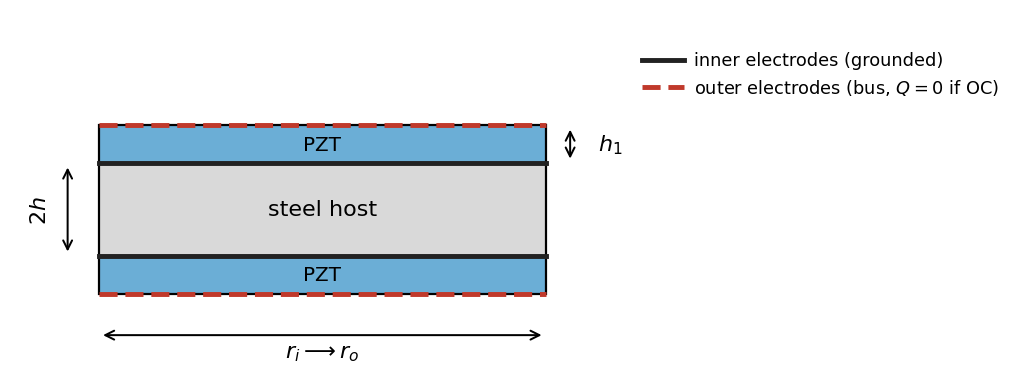
\includegraphics[width=0.92\linewidth]{piezo_p4_geometry.png}
\caption{Radial--thickness slice of the layered annulus (not to scale).
Inner electrodes sit at $z=\pm h$ and are grounded. Outer electrodes at
$z=\pm(h+h_1)$ are shorted to the inners under short-circuit, and form a
single unconstrained bus with $Q=0$ under open-circuit.}
\label{fig:geom}
\end{figure}

Kirchhoff kinematics $u_z=w(r,\theta,t)$ in the host, with the usual
plane-stress reduction of each piezo layer, produce the reduced constants
\begin{equation}
\eebar = e_{31}-\frac{c_{13}^E}{c_{33}^E}e_{33},\qquad
\Xibar = \Xi_{33}+\frac{e_{33}^2}{c_{33}^E}.
\label{eq:reduced}
\end{equation}
For the PZT-4 values above, $\eebar=-4.85\,\mathrm{C\,m^{-2}}$: the
$c_{13}^E e_{33}/c_{33}^E$ correction exceeds $e_{31}$ itself, so the
sign of the reduced constant is opposite the tabulated $e_{31}$. Duan,
Quek and Wang's own tables print $e_{31}=-4.1\,\mathrm{C\,m^{-2}}$; the
$+4.1$ used here is a deliberate sign convention consistent with this
group's related work, not a correction to their value or a discrepancy
to be reconciled. Bending
stiffness splits into a host contribution and a purely elastic
contribution from the two layers,
\begin{equation}
d_1=\frac{2}{3}\frac{E h^3}{1-\nu^2},\qquad
\bar c_{11}=c_{11}^E-\frac{(c_{13}^E)^2}{c_{33}^E},\qquad
d_2=\frac{2}{3}\bar c_{11}\bigl[(h+h_1)^3-h^3\bigr].
\label{eq:d1d2}
\end{equation}
The electromechanical moment is proportional to $\eebar$ times the
through-thickness electric field. The term $d_2$ is present whether the
electrodes are open or shorted; it is ordinary added-layer stiffness,
and it is what Duan, Quek and Wang's Fig.~3 isolates as the dominant
short-circuit frequency shift.

\section{Short-circuit determinant}\label{sec:sc}
Short-circuit electrodes on both faces of each layer are encoded by an
interior potential that vanishes on both faces of the layer,
\begin{equation}
\varphi=\bar\varphi(r,\theta,t)\,\frac{4(z-h)(h+h_1-z)}{h_1^2}
\label{eq:sine}
\end{equation}
in the top layer, with its mirror below, so $\varphi=0$ at $z=\pm h$ and
at $z=\pm(h+h_1)$. The equation for $\bar\varphi$ is the stationarity
condition of the thickness-integrated electric enthalpy, the same
Galerkin projection that produces the flexural equation. Duan, Quek and
Wang \cite{duan2005} used a sinusoidal profile,
$\sin(\pi(z-h)/h_1)$, and closed its electrical equation instead by
integrating Gauss's law through the layer; that closure is not conjugate
to the moment through which the coupling reaches the flexural equation,
and in the long-wave limit it overstates each layer's own short-circuit
stiffening, $h_1^3\eebar^{\,2}/(12\Xibar)$, by exactly $12/\pi^2$. The
quadratic \eqref{eq:sine} is the one-term profile whose projected
long-wave stiffening is exact (Supplementary~\S S.1). On this
steel-dominated stack the difference is invisible at Table~4's printed
precision (the largest root moves by $0.0015\%$). Substituting
\eqref{eq:sine} into the flexural operator and the projected electrical
equation, and positing
$\bar\varphi=\chi w$ with $\chi$ independent of $r$, produces two
Helmholtz equations for $w$ that are simultaneously satisfiable only
when $\chi$ and the radial eigenvalue $\lambda$ obey a cubic consistency
condition (Supplementary~\S S.1). The cubic has three roots
$(\chi_i,\lambda_i)$, $i=1,2,3$, each a function of the trial frequency
$\omega$. For each root the radial problem is second-order Helmholtz,
with Bessel pair $(J_n,Y_n)$ or modified pair $(I_n,K_n)$ according to
the sign of $\lambda_i$. Three branches times two radial functions is a
six-dimensional basis, matching the sixth-order coupled system. The
general solution is a sum over all three branches.

Edge conditions per radius are mechanical plus the insulated-edge
condition $\partial\varphi/\partial r=0$. The six rows of the
short-circuit matrix, in order, are
\begin{equation}
\begin{aligned}
&\text{clamped--clamped:}
 &&w,\; w',\; \partial\varphi/\partial r
 &&\text{at }r=r_i\text{ and }r=r_o,\\
&\text{free--free:}
 &&M_{rr},\; Q_r^{\mathrm{eff}},\; \partial\varphi/\partial r
 &&\text{at }r=r_i\text{ and }r=r_o.
\end{aligned}
\label{eq:rows}
\end{equation}
Here $Q_r^{\mathrm{eff}}=Q_r+r^{-1}\partial M_{r\theta}/\partial\theta$ is the
Kirchhoff effective shear. The twisting moment $M_{r\theta}$ carries no
piezoelectric term, and the correction it adds to $Q_r$ is proportional
to $n^2$, so $Q_r^{\mathrm{eff}}=Q_r$ at $n=0$.
Either pair is a $6\times6$ determinant. Zeros
are found by a real-part sign-flip bisection on a pre-registered
frequency bracket, with a negative-control bracket that is not allowed
to flip. Published frequencies never seed a search; they enter only when
a converged root is scored against them.

Setting $\eebar\to0$ is a singular limit of the cubic (the leading
coefficient and two subleading coefficients vanish together), so the
elastic bilayer $d_1+d_2$ is assembled as a separate two-branch
$4\times4$, not by zeroing $\eebar$ inside the $6\times6$. That
$4\times4$ is the short-circuit operator of the linear-potential model
in \S\ref{sec:oc}, because $V=0$ implies $E_z=0$ and $M_p=0$.

\section{Open-circuit determinant}\label{sec:oc}
Open-circuit of the same fully electroded stack is not a flag on the
$6\times6$. Inner electrodes (the host/piezo interfaces) remain grounded,
because the host is a conductor. Outer electrodes form a conducting bus
at unknown voltage $V(t)$, spatially constant, with total charge $Q=0$.
The leading through-thickness field is then linear,
\begin{equation}
\varphi_{\mathrm{top}}=V\frac{z-h}{h_1},\qquad
\varphi_{\mathrm{bottom}}=-V\frac{z+h}{h_1},
\label{eq:linpot}
\end{equation}
for a same-poling parallel bimorph. Laboratory $E_z$ is opposite in the
two layers, extra in-plane stresses are opposite, and the moments
\emph{add}:
\begin{equation}
M_p=2\eebar\bigl(h+h_1/2\bigr)V,
\label{eq:Mp}
\end{equation}
spatially constant. A constant isotropic moment does not enter $Q_r^{\mathrm{eff}}$ or
the interior plate operator. It enters only the natural condition
$M_{rr}=0$.

The bus charge on both outers is the variable conjugate to $V$ in the
same electric enthalpy,
\begin{equation}
Q=2\eebar(h+h_1/2)\int_A\nabla^2 w\,\mathrm{d}A+C_0 V,\qquad
C_0=\frac{2\Xibar A}{h_1},\qquad
A=\pi(r_o^2-r_i^2).
\label{eq:Q}
\end{equation}
Its motional arm $h+h_1/2$ is the layer mid-surface, the same arm as
$M_p$ in \eqref{eq:Mp}, so the open-circuit operator is reciprocal; in
the exact thin-plate solution $D_z$ is uniform through each layer and
couples only to the layer's mean strain. Evaluating the linear field's
$D_z$ at the outer electrode instead gives the arm $h+h_1$, which
overstates every open-circuit split below by $(h+h_1)/(h+h_1/2)$
($7.7\%$, $11\%$, and $17\%$ at the three Table~4 ratios). The interior
potential \eqref{eq:sine} contributes no bus charge, because its field
integrates to zero across each layer. Green's identity on the annulus
gives $\int_A\nabla^2 w\,\mathrm{d}A=2\pi S$ at $n=0$, with
$S=r_o w'(r_o)-r_i w'(r_i)$, and vanishes at $n\neq0$ by the
$\theta$-integral. Open-circuit $Q=0$ therefore determines $V$ from $S$
when $n=0$, and is vacuous when $n\neq0$. Substituting into $M_{rr}=0$
produces a rank-1 update of the elastic free--free $4\times4$: both
$M_{rr}$ rows receive $\alpha S$,
\begin{equation}
\alpha=\frac{4\eebar^2 (h+h_1/2)^2h_1}{\Xibar(r_o^2-r_i^2)},
\label{eq:alpha}
\end{equation}
the $Q_r^{\mathrm{eff}}$ rows are unchanged, and the sign $+\alpha$ is the one that
raises the $n=0$ root. For $n\neq0$ or $h_1=0$ the update is identically
zero. That is not a numerical observation: at $h_1/2h=1/12$ the first
free--free $n=1$ root of the open-circuit $4\times4$ is bit-identical to
the elastic bilayer, $1756.00\,\mathrm{rad\,s^{-1}}$. A continuous
electrode cannot collect net charge from a nodal-diameter mode.

\subsection{Clamped--clamped open-circuit is short-circuit}
\label{sec:theorem}
If $w'=0$ on the entire boundary, Green's identity forces
$\int_A\nabla^2 w\,\mathrm{d}A=0$. Equation~\eqref{eq:Q} collapses to
$Q=C_0 V$, so $Q=0$ implies $V=0$. Clamped--clamped open-circuit
coincides with short-circuit, and with the elastic bilayer, at this
order. The only remaining clamped--clamped coupling is the interior
potential already in the $6\times6$, whose frequency effect is $0.01\%$ in Duan,
Quek and Wang's Fig.~3 \cite{duan2005}. A frequency-based inverse for
$e_{31}$ from a clamped--clamped short-circuit mode is therefore asking
a $0.01\%$ correction to identify a constitutive constant.
Section~\ref{sec:inverse} measures that as an $889\%$ uncertainty at
$0.01\%$ frequency precision. Switching the same mode to open-circuit
does not help. Free--free axisymmetric motion does: $S\neq0$ in general,
$V$ is alive, and $M_p$ is seen by $M_{rr}=0$. A mixed mechanical edge
is the intermediate case. Clamped inner and free outer (C--F; Paper~3's
inner-then-outer naming) forces $w'(r_i)=0$, so $S=r_o w'(r_o)$ on the
mode and the rank-1 update lives only on the outer $M_{rr}$ row.
Free inner and clamped outer (F--C) is the swap. Neither is a
coincidence theorem: one edge remains free, so $S$ need not vanish.

\section{Forward validation}\label{sec:forward}
\subsection{Clamped--clamped short-circuit against Table~4}
\label{sec:table4}
Table~\ref{tab:duan} reports every non-trivial point of Duan, Quek and
Wang's Table~4 \cite{duan2005}: circumferential orders $p=0,1,2$, the
first three radial indices, and the three thickness ratios. Targets are
the printed integers. The $6\times6$ is searched from scratch; a
pre-registered relative bar of $0.15\%$ is applied after the fact and is
not used to retune a root. All 27 points pass. The worst relative error
is $-0.0490\%$, at $p=2$, first radial, $h_1/2h=1/5$. Duan, Quek and
Wang's own sine closure reproduces the same 27 points (worst
$-0.0476\%$), and no root differs between the two closures by more
than $0.0015\%$. The integer-Hz
table does not resolve the $0.01\%$ electromechanical correction, so
this comparison confirms the layered Kirchhoff operator including
added-layer stiffness, not the open-circuit splitting of
\S\ref{sec:ffoc}.

\begin{table}[H]
\centering
\caption{Clamped--clamped short-circuit frequencies ($\mathrm{rad\,s^{-1}}$)
against Duan, Quek and Wang Table~4 \cite{duan2005}. $p$ is
circumferential order; $s$ is radial index as in that table. Bar:
$0.15\%$. All 27 pass.}
\label{tab:duan}
\small
\begin{tabular}{@{}rrrcccc@{}}
\toprule
$p$ & $s$ & $h_1/2h$ & Table~4 & present & rel.\ \% \\
\midrule
0 & 0 & $1/12$ & 2792 & 2791.78 & $-0.0078$ \\
0 & 0 & $1/8$  & 2853 & 2852.18 & $-0.0286$ \\
0 & 0 & $1/5$  & 2989 & 2987.69 & $-0.0437$ \\
0 & 1 & $1/12$ & 7723 & 7722.70 & $-0.0039$ \\
0 & 1 & $1/8$  & 7891 & 7889.78 & $-0.0155$ \\
0 & 1 & $1/5$  & 8268 & 8264.63 & $-0.0407$ \\
0 & 2 & $1/12$ & 15182 & 15181.11 & $-0.0058$ \\
0 & 2 & $1/8$  & 15512 & 15509.56 & $-0.0157$ \\
0 & 2 & $1/5$  & 16253 & 16246.44 & $-0.0404$ \\
1 & 0 & $1/12$ & 2928 & 2928.22 & $+0.0074$ \\
1 & 0 & $1/8$  & 2992 & 2991.57 & $-0.0144$ \\
1 & 0 & $1/5$  & 3135 & 3133.70 & $-0.0413$ \\
1 & 1 & $1/12$ & 7965 & 7964.36 & $-0.0080$ \\
1 & 1 & $1/8$  & 8138 & 8136.67 & $-0.0163$ \\
1 & 1 & $1/5$  & 8527 & 8523.26 & $-0.0439$ \\
1 & 2 & $1/12$ & 15482 & 15480.88 & $-0.0073$ \\
1 & 2 & $1/8$  & 15818 & 15815.81 & $-0.0139$ \\
1 & 2 & $1/5$  & 16574 & 16567.24 & $-0.0408$ \\
2 & 0 & $1/12$ & 3477 & 3477.17 & $+0.0048$ \\
2 & 0 & $1/8$  & 3553 & 3552.40 & $-0.0170$ \\
2 & 0 & $1/5$  & 3723 & 3721.17 & $-0.0490$ \\
2 & 1 & $1/12$ & 8768 & 8768.04 & $+0.0004$ \\
2 & 1 & $1/8$  & 8959 & 8957.73 & $-0.0141$ \\
2 & 1 & $1/5$  & 9387 & 9383.33 & $-0.0391$ \\
2 & 2 & $1/12$ & 16434 & 16433.67 & $-0.0020$ \\
2 & 2 & $1/8$  & 16791 & 16789.22 & $-0.0106$ \\
2 & 2 & $1/5$  & 17594 & 17586.89 & $-0.0404$ \\
\bottomrule
\end{tabular}
\end{table}

\subsection{Free--free open-circuit, three thickness ratios}
\label{sec:ffoc}
No literature table exists for free--free piezoelectric rings. Closed
form is still exact. Table~\ref{tab:ff} reports the first $n=0$ flexural
root of the elastic bilayer, of the short-circuit $6\times6$, and of the
open-circuit rank-1 $4\times4$, at all three of Duan, Quek and Wang's Table~4 thickness ratios.
Short-circuit coupling on this mode is $+0.00072\%$ to $+0.0073\%$
relative to the bilayer: that is Duan, Quek and Wang's Fig.~3 in
numbers. Open-circuit coupling is two orders of magnitude larger, and it
grows with $h_1/2h$: $+0.280\%$, $+0.405\%$, $+0.601\%$. Thicker layers
put more of the bending stiffness in the piezo and give the rank-1
moment a longer lever arm, so the identifying split is not a property of
one geometry. A closed-form sweep of eleven ratios from $h_1/2h=1/40$
to $1/4$ places those three of Duan, Quek and Wang's Table~4 points on a smooth curve
(Supplementary Fig.~S.2). As $h_1/2h\to0$ the split is linear in layer
thickness: $\Delta_{\mathrm{OC}}/(h_1/2h)\to 0.035$. The same sweep
turns the three-point open-circuit $e_{31}$ column of
Table~\ref{tab:inv} into a curve: $0.01\%$ frequency precision maps to
$6.80\%$ of $e_{31}$ at $1/40$ and $0.85\%$ at $1/4$. The first $n=0$
radial overtone still splits, but more weakly: $3504.95$ vs
$3509.42\,\mathrm{rad\,s^{-1}}$ ($+0.128\%$, $k_{\mathrm{eff}}^2=0.00255$),
and $0.01\%$ frequency precision maps to $4.66\%$ of $e_{31}$. The next
sits at $8515.06$ vs $8516.38\,\mathrm{rad\,s^{-1}}$ ($+0.016\%$,
$38\%$ of $e_{31}$ at $0.01\%$ frequency). The identifying observable
remains the fundamental.

\begin{table}[H]
\centering
\caption{First free--free $n=0$ flexural frequency. Closed-form values
in $\mathrm{rad\,s^{-1}}$ (Hz in parentheses). $\Delta_{\mathrm{OC}}$
is the rank-1 $4\times4$ relative to the elastic bilayer. Short-circuit
$6\times6$ coupling on this mode is $+0.00072\%$ to $+0.0073\%$ and is
omitted from the last column.}
\label{tab:ff}
\small
\begin{tabular}{@{}lcccc@{}}
\toprule
$h_1/2h$ & bilayer & SC $6\times6$ & OC $4\times4$ & $\Delta_{\mathrm{OC}}$ \\
\midrule
$1/12$ & 747.986 (119.046) & 747.992 (119.047) & 750.079 (119.379) & $+0.280\%$ \\
$1/8$  & 764.113 (121.612) & 764.130 (121.615) & 767.209 (122.105) & $+0.405\%$ \\
$1/5$  & 800.303 (127.372) & 800.361 (127.381) & 805.112 (128.138) & $+0.601\%$ \\
\bottomrule
\end{tabular}
\end{table}

External confirmation at $h_1/2h=1/12$ is axisymmetric coupled-field
finite elements (PLANE223, KEYOPT(1)=1001) on one mesh, in the
millimetre--newton--second--tonne system with relative permittivity.
Coupling-off ($e_{ij}=0$) gives $118.810\,\mathrm{Hz}$. Both-faces
short-circuit (VOLT$=0$ on $z=\pm h$ and $z=\pm(h+h_1)$) gives
$118.811\,\mathrm{Hz}$, matching coupling-off to $+0.0007\%$ and
confirming that true short-circuit on this mode is the bilayer.
Open-circuit (VOLT$=0$ on the interfaces; one coupled VOLT set on both
outer faces, unconstrained) gives $119.143\,\mathrm{Hz}$. The
finite-element split relative to true short-circuit is $+0.279\%$,
against the closed-form $+0.280\%$ (ratio $0.999$). Both modes are bending:
transverse displacement has the same sign through the thickness at
$r=r_o$, radial displacement is opposite, and the ratio of those
components is $19.71$ (short-circuit) and $19.75$ (open-circuit). A deck
that grounds only the outer faces and leaves the interface free sits at
$119.242\,\mathrm{Hz}$ and is a mixed electrical condition, $0.36\%$
above true short-circuit; it is not used as the short-circuit baseline
(Supplementary~\S S.3).

The same fair pair, cloned without remeshing to the other two Table~4
ratios, confirms the same stiffening trend. At $h_1/2h=1/8$,
open-circuit gives $121.839\,\mathrm{Hz}$ against $121.348\,\mathrm{Hz}$
both-faces short-circuit, a $+0.405\%$ split against the closed-form
$+0.405\%$; at $h_1/2h=1/5$, $127.809\,\mathrm{Hz}$ against
$127.047\,\mathrm{Hz}$, a $+0.600\%$ split against the closed-form
$+0.601\%$. Every deck shows the same bending signature
(ratio of thickness-through components $19.7$--$19.8$) and a $0\,\mathrm{Hz}$
rigid-body mode, and no run printed an element-level error. The
finite-element split is $99.9\%$, $99.9\%$, and $99.8\%$ of the
closed-form split. An earlier version of this model took the bus charge
from $D_z$ at the outer electrode (arm $h+h_1$); finite elements then
recovered $93\%$, $90\%$, and $86\%$ of its splits, which is
$(h+h_1/2)/(h+h_1)$ at each ratio to within $0.5\%$ and is how the
non-reciprocal charge row was found. Doubling the piezo through-thickness
divisions on the same electrical pair leaves the three finite-element
splits unchanged at the printed precision.

\paragraph{Three-dimensional check at $n\ge1$.} The finite-element
models above are axisymmetric, so they see $n=0$ only. A
three-dimensional coupled-field model (SOLID226 half ring,
$0\le\theta\le\pi$ with a symmetric cut, so every $\cos n\theta$ order
appears in one solve; same materials, units, and electrical conditions)
was run at $h_1/2h=1/12$ and $1/5$ on two meshes
(Supplementary~\S S.9). Its $n=0$ roots reproduce the axisymmetric
ones: coupling-off $118.8105$ against $118.8102\,\mathrm{Hz}$, and
open-/short-circuit splits of $0.2796\%$ and $0.6002\%$ against
$0.2795\%$ and $0.6002\%$. At $n=1$--$4$ it gives three results. Open
circuit coincides with short circuit to $10^{-10}$ relative, with a bus
voltage below $10^{-9}$ of its $n=0$ value, as the no-net-charge
argument of \S\ref{sec:oc} requires. The short-circuit stiffening from
the interior potential, $1.4\times10^{-6}$ to $7.3\times10^{-5}$
relative and non-monotone in $n$, is reproduced to within $1.2\%$ of
the $6\times6$ value at every $n=0$--$4$ and both ratios; that is the
coupled $n\ge1$ content of the model, and nothing else checks it. The
elastic roots themselves sit $0.53\%$ to $1.19\%$ below the thin-plate
values at $n=1$--$4$, against $0.20\%$ and $0.26\%$ at $n=0$: one-signed,
mesh-converged to $0.03\%$, largest at $n=1$, and larger for the
thicker layer at every $n$ -- the same pattern as the free--free
shell-element comparison of \cite{mccune2026ring}. It is a thickness
effect, not an error in the $n\ge1$ operator: on a bare steel annulus of
the same planform at $20$, $10$ and $5\,\mathrm{mm}$, with the mesh
error removed by Richardson extrapolation over three uniformly refined
meshes, the $n=1$--$4$ offset falls from $0.49$--$0.92\%$ to
$0.11$--$0.16\%$, and its extrapolation to zero thickness is within
$0.015\%$ of zero at every $n=0$--$4$ (Supplementary~\S S.9). The $n=0$
offset is purely quadratic in thickness; at $n\ge1$ a first-order term
of comparable or larger size appears, as expected of the free-edge
boundary layer that a Kirchhoff effective-shear edge omits. The superseded $Q_r$ free-edge row put $n=1$ at
$h_1/2h=1/12$ at $1573.49\,\mathrm{rad\,s^{-1}}$; the three-dimensional
root is $10.5\%$ above it, and $1.0\%$ below the effective-shear value.

\subsection{Clamped--free and free--clamped open-circuit}
\label{sec:cf}
The elastic mixed-edge $4\times4$ is Paper~3's construction
\cite{mccune2026ring}: C--F replaces the inner $M_{rr}$ and $Q_r^{\mathrm{eff}}$ rows
by $w=w'=0$; F--C is the swap. At $h_1=0$ those determinants recover
the live Paper~3 ring solver on this geometry to $4.5\times10^{-10}$
(C--F) and $2.3\times10^{-10}$ (F--C) relative. Short-circuit coupling
on the mixed $6\times6$ remains the usual interior-potential correction,
$+0.00084\%$ (C--F) and $+0.00054\%$ (F--C) at $h_1/2h=1/12$.
Open-circuit does not coincide with that bilayer. Table~\ref{tab:cf}
records the first $n=0$ root. C--F splits by $+0.262\%$
($k_{\mathrm{eff}}^2=0.00522$), comparable to the free--free
$+0.280\%$ at the same ratio, because the free outer radius still
carries $S=r_o w'(r_o)$. F--C splits by $+0.00538\%$
($k_{\mathrm{eff}}^2=0.000108$): only the inner hole is free, so
$S=-r_i w'(r_i)$ and the rank-1 moment acts on the smaller edge.
$n\neq0$ open-circuit is bit-identical to the mixed elastic $4\times4$
on both pairs, as for free--free. Axisymmetric finite elements on the
same mesh as \S\ref{sec:ffoc}, with only the inner radius clamped
($U_X=U_Y=0$ through the stack, outer free), confirm the C--F split:
both-faces short-circuit $67.071\,\mathrm{Hz}$ against open-circuit
$67.245\,\mathrm{Hz}$, $+0.259\%$, against the closed-form $+0.262\%$
(ratio $0.989$). No $0\,\mathrm{Hz}$ rigid body (the clamp took). Both
modes are bending ($U_Y$ same sign through the thickness at $r=r_o$,
$U_X$ opposite, ratio $\approx 45.6$). F--C was not meshed.

\begin{table}[H]
\centering
\caption{First $n=0$ mixed-edge flexural frequency at $h_1/2h=1/12$,
closed form, $\mathrm{rad\,s^{-1}}$ (Hz). C--F is inner clamped, outer
free; F--C is the swap. $\Delta_{\mathrm{OC}}$ is relative to the
mixed-edge elastic bilayer.}
\label{tab:cf}
\small
\begin{tabular}{@{}lcccc@{}}
\toprule
edge & bilayer & SC $6\times6$ & OC $4\times4$ & $\Delta_{\mathrm{OC}}$ \\
\midrule
C--F & 421.895 (67.147) & 421.898 (67.147) & 423.001 (67.323) & $+0.262\%$ \\
F--C & 899.061 (143.090) & 899.066 (143.091) & 899.110 (143.098) & $+0.00538\%$ \\
\bottomrule
\end{tabular}
\end{table}

\FloatBarrier
\section{Inverse recovery}\label{sec:inverse}
The unknown is a single material constant $p$; every other constant is
held at its true value. A target $\omega_\star$ is the exact forward
root at $p_{\mathrm{true}}$. The residual
$G(p)=\omega_{\mathrm{root}}(p)-\omega_\star$ is bisected on a bracket
that contains a genuine sign flip; a hi-side-only bracket is the
negative control. On-branch finite differences give
$\mathrm{d}p/\mathrm{d}\omega$, hence the uncertainty in $p$ at an
assumed relative precision in $\omega$. The same recipe inverted
Southwell's $b/a$ at fixed $\lambda^2$ for the elastic ring
\cite{mccune2026ring}. Round-trip recovery of $p_{\mathrm{true}}$ from
$\omega_\star$ is $4\times10^{-9}$ relative against a $10^{-6}$ bar in
every case below; the inverse machinery is not the issue. The scientific
content is the propagated uncertainty.

Table~\ref{tab:inv} records host $E$ from the clamped--clamped
short-circuit fundamental at $h_1/2h=1/12$, and $e_{31}$ from that same
short-circuit family and from the free--free and clamped--free
open-circuit $n=0$ roots, at
all three thickness ratios for free--free and at $h_1/2h=1/12$ for
clamped--free. Host $E$ is well conditioned under
short-circuit, as required by $\omega\sim\sqrt{E}$ (relative $E$
uncertainty $\approx 2$ times frequency precision). Short-circuit
$e_{31}$ is not: $0.01\%$ in frequency becomes $889\%$, $294\%$, and
$88\%$ in $e_{31}$ as the layer thickens. Open-circuit reduces those
figures to $2.13\%$, $1.48\%$, and $1.00\%$. Clamped--free open-circuit
at $h_1/2h=1/12$ is $2.28\%$, the same class as free--free.
Thickness helps both
electrical conditions, because more of the bending stiffness sits in the
piezo, but it does not close the electrical gap: at $h_1/2h=1/5$
short-circuit is still two orders of magnitude worse than open-circuit.
Figure~\ref{fig:id} is the same comparison.

Those open-circuit figures hold $E$ at its true value, which no
experiment can do. The last row of Table~\ref{tab:inv} instead recovers
$E$ from the clamped--clamped short-circuit fundamental first, then
$e_{31}$ from the free--free open-circuit root using that recovered
$\hat E$, and propagates $\hat E$'s own uncertainty forward into
$e_{31}$ -- the two-step protocol an actual measurement would follow, at
$h_1/2h=1/12$. The result is $3.01\%$ of $e_{31}$ at $0.01\%$ frequency
precision: a direct term of $2.13\%$, matching the idealized row above,
plus an almost equally large term of $2.12\%$ from propagating $\hat E$'s
own $0.025\%$ uncertainty through the open-circuit root's weak but
nonzero dependence on $E$. Substituting the clamped--clamped open-circuit
root for the free--free one in the second step -- the negative
control -- reproduces the $889\%$ short-circuit figure instead
($888.5\%$), confirming that the sequential protocol still requires the
free--free open-circuit observable and gains nothing from the
clamped--clamped one.
Host $E$ recovered from free--free $n=0$ elastic or open-circuit
flexure is the same thermometer as the clamped--clamped short-circuit
channel to the printed digit ($0.025\%$ at $0.01\%$ frequency). From
the same open-circuit fundamental, host $\nu$ and the piezo-layer
$C_{11}^E$ recover at $0.107\%$ and $0.072\%$; $\Xi_{33}$ from that
frequency is $4.67\%$, while the clamped capacitance $C_0$ identifies
$\Xi_{33}$ at roundoff. Frequency is a poor dielectric thermometer;
$C_0$ is the one.

\begin{table}[H]
\centering
\caption{Single-parameter inverse. Round-trip relative error on
$p_{\mathrm{true}}$ is $4\times10^{-9}$ in every row (bar $10^{-6}$).
Propagated relative uncertainty is at $0.01\%$ frequency precision.
C--C SC: clamped--clamped short-circuit fundamental. F--F OC: free--free
open-circuit, $n=0$. C--F OC: clamped-inner, free-outer open-circuit,
$n=0$. The three $E$ rows are independent channels of the
same $\omega\sim\sqrt{E}$ thermometer. The last row recovers $E$ from
the first row, then $e_{31}$ from the F--F OC $e_{31}$ row, propagating
$\hat E$'s uncertainty forward.}
\label{tab:inv}
\small
\begin{tabular}{@{}llr@{}}
\toprule
forward model & unknown & unc.\ at $0.01\%$ freq. \\
\midrule
C--C SC, $h_1/2h=1/12$ & $E=2\times10^{11}\,\mathrm{Pa}$ & $0.025\%$ of $E$ \\
F--F elastic, $h_1/2h=1/12$ & $E$ & $0.025\%$ of $E$ \\
F--F OC, $h_1/2h=1/12$ & $E$ & $0.025\%$ of $E$ \\
C--C SC, $h_1/2h=1/12$ & $e_{31}$ & $889\%$ of $e_{31}$ \\
C--C SC, $h_1/2h=1/8$  & $e_{31}$ & $294\%$ of $e_{31}$ \\
C--C SC, $h_1/2h=1/5$  & $e_{31}$ & $88\%$ of $e_{31}$ \\
F--F OC, $h_1/2h=1/12$ & $e_{31}$ & $2.13\%$ of $e_{31}$ \\
C--F OC, $h_1/2h=1/12$ & $e_{31}$ & $2.28\%$ of $e_{31}$ \\
F--F OC, $h_1/2h=1/8$  & $e_{31}$ & $1.48\%$ of $e_{31}$ \\
F--F OC, $h_1/2h=1/5$  & $e_{31}$ & $1.00\%$ of $e_{31}$ \\
F--F OC (seq.\ $\hat E$), $h_1/2h=1/12$ & $e_{31}$ & $3.01\%$ of $e_{31}$ \\
\bottomrule
\end{tabular}
\end{table}

\begin{figure}[ht]
\centering
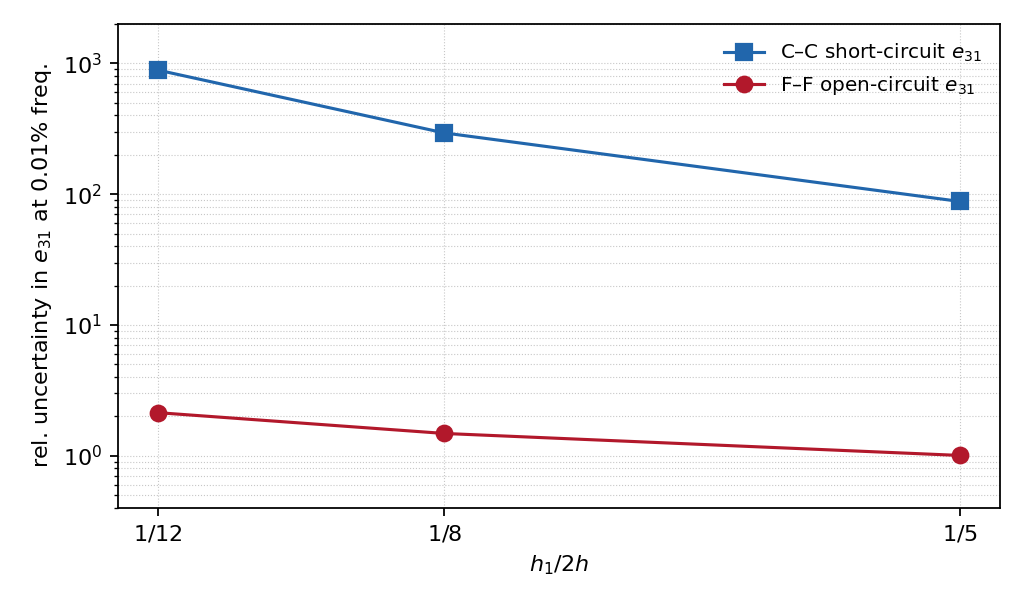
\includegraphics[width=0.92\linewidth]{piezo_p4_identifiability.png}
\caption{Propagated relative uncertainty in $e_{31}$ at $0.01\%$
frequency precision, on the clamped--clamped short-circuit fundamental
and on the free--free open-circuit $n=0$ root. Both improve as $h_1/2h$
grows; the electrical gap does not close.}
\label{fig:id}
\end{figure}

Two caveats sit on the open-circuit inverse. First, $\omega_{\mathrm{OC}}$
depends on $\eebar^2$, so a frequency determines $|\eebar|$ and therefore
two raw $e_{31}$ values reflected about $(c_{13}^E/c_{33}^E)e_{33}\approx 8.95\,\mathrm{C\,m^{-2}}$.
Duan, Quek and Wang's $e_{31}=4.1$ is the lower branch; the twin is near
$13.8\,\mathrm{C\,m^{-2}}$, outside the bracket used here. Holding
$e_{33}$ known, as a single-parameter recovery requires, selects the
branch. A joint $(e_{31},e_{33})$ fit would re-open the reflection.
Second, a joint $(E,e_{31})$ fit from one short-circuit frequency would
be worse than the $e_{31}$-only short-circuit row, not better: one
well-conditioned parameter cannot regularize an unidentifiable one.
Additional short-circuit flexural modes of the same family will not
collapse the $889\%$ figure, because they share the same $0.01\%$
coupling. Open-circuit on a clamped--clamped mode will not either, by
\S\ref{sec:theorem}. The identifying observable for $e_{31}$ is an
axisymmetric open-circuit frequency on a plate that has at least one
free edge: the free--free $n=0$ root, or the C--F $n=0$ root of
Table~\ref{tab:cf} ($2.28\%$ of $e_{31}$ at $0.01\%$ frequency, against
free--free's $2.13\%$). F--C open-circuit is not: its $0.0054\%$ split
is two orders of magnitude smaller, and is a result, not a failed
search.

The $2.13\%$/$2.28\%$ figures above assume $0.01\%$ frequency
precision, an optimistic narrow-band-tracking number rather than a
measured instrument comparison. Figure~\ref{fig:noisefloor} extends
the free--free and clamped--free open-circuit inverse along the
frequency-precision axis itself, rather than reporting only the two
columns of Table~\ref{tab:inv}: the propagated relative uncertainty
in $e_{31}$ is linear in the assumed relative frequency error over
three decades, by construction of the linear-propagation formula, so
there is no threshold below which the recovery qualitatively changes
and no floor at which it saturates. A lab-realistic floor, taken as
the impedance-analyzer-versus-scanning-laser-Doppler-vibrometer
frequency disagreement measured on a physically distinct PZT rod
specimen in companion experimental work from this group
\cite{boeringa2026} (mean $0.10\%$ across five axial modes), lands
within a few percent of the already-tabulated $0.1\%$ column for both
channels ($21.8\%$ and $23.2\%$ of $e_{31}$, against $21.3\%$ and
$22.8\%$). The gap between the idealized $0.01\%$ precision and this
cross-instrument comparison, not the choice between the free--free and
clamped--free observables (which agree with each other to within about
$7\%$ at every precision tested), is the dominant source of
uncertainty in a real inverse recovery.

\begin{figure}[ht]
\centering
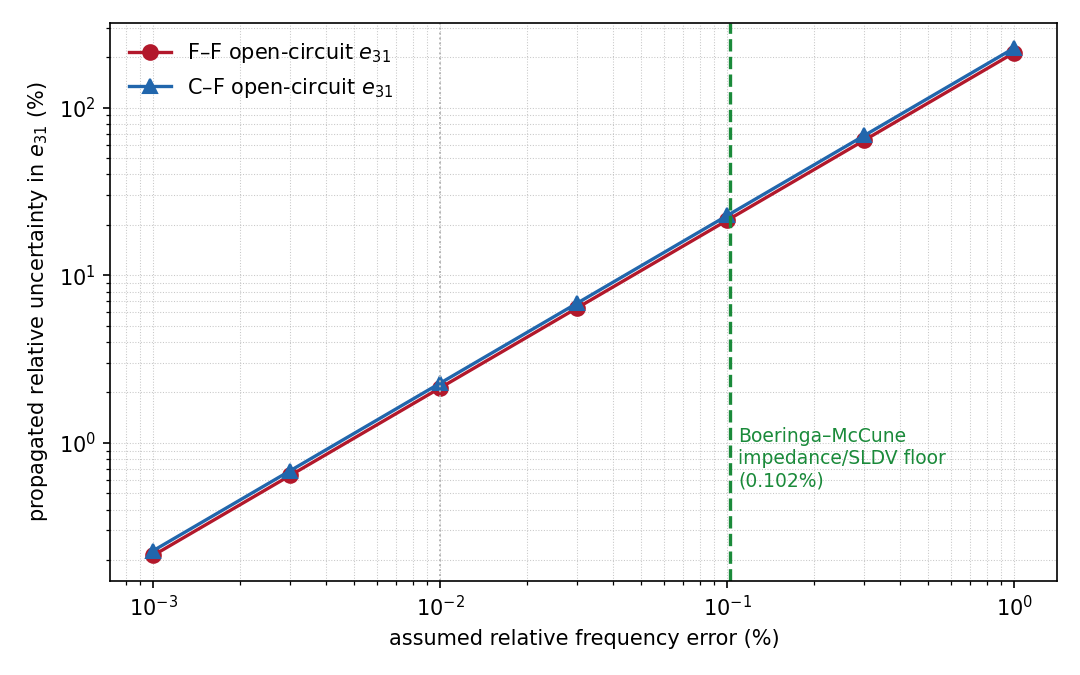
\includegraphics[width=0.92\linewidth]{piezo_p4_lever16_noise_floor.png}
\caption{Propagated relative uncertainty in $e_{31}$ versus assumed
relative frequency error, free--free and clamped--free $n=0$
open-circuit. Linear on log--log axes by construction of the
propagation formula. The dashed line marks the
impedance-analyzer/SLDV frequency-disagreement floor measured on a
physically distinct rod specimen \cite{boeringa2026}, which coincides
closely with the already-tabulated $0.1\%$ column.}
\label{fig:noisefloor}
\end{figure}

Read as a measurement promise, $2.13\%$ (F--F) and $2.28\%$ (C--F)
at $0.01\%$ frequency precision would require resolving these
resonances to one part in ten thousand -- finer than the
impedance-analyzer/SLDV comparison of Fig.~\ref{fig:noisefloor}
delivers on a physically similar specimen. Read instead as a
statement about well-posedness, the result stands regardless of
instrument: $\mathrm{d}\omega_{\mathrm{OC}}/\mathrm{d}e_{31}$ is
nonzero and large enough that \emph{any} finite frequency measurement
maps to a finite $e_{31}$ interval, in contrast to the short-circuit
clamped--clamped channel, where the same derivative is so small that
no realistic frequency precision recovers $e_{31}$ at all ($889\%$ at
$0.01\%$, worse at any coarser floor). The $0.01\%$ column is
therefore best read as characterizing the conditioning of the inverse
problem -- how tightly a well-resolved frequency constrains
$e_{31}$ -- rather than as a laboratory accuracy target; the number an
actual bench measurement on this ring would deliver is closer to the
Boeringa--McCune floor, roughly $22\%$. Both readings support the same
qualitative conclusion, that the open-circuit observable unlocks
$e_{31}$ where short-circuit cannot; only the second is the number to
quote for what a real experiment on such a ring would recover.

\section{Driven admittance}\label{sec:Y}
Imposing $V$ rather than $Q=0$ converts \S\ref{sec:oc} into a driven
problem: the elastic $4\times4$ is solved with $M_{rr}$-row right-hand
side $M_p$ at both edges, and $Q$ follows from \eqref{eq:Q}. The undamped
admittance is $Y(\omega)=j\omega Q/V$, or equivalently the real effective
capacitance $C_{\mathrm{eff}}(\omega)=Q/V$. For $n\neq0$, $S=0$ and
$C_{\mathrm{eff}}=C_0$ identically: a continuous electrode carries no
net motional charge in a nodal-diameter mode. For $n=0$,
$C_{\mathrm{eff}}$ has a pole at the short-circuit (elastic) root and a
zero at the open-circuit root. An independent bisection of $Q/V$ at
$h_1/2h=1/12$ recovers $750.0794987774\,\mathrm{rad\,s^{-1}}$ at a
relative difference of $1.4\times10^{-15}$ from the free-vibration
$4\times4$. The IEEE coupling factor \cite{ieee176} built from those two
frequencies is
\begin{equation}
k_{\mathrm{eff}}^{2}=1-(f_{r}/f_{a})^{2}.
\label{eq:keff}
\end{equation}
At $h_1/2h=1/12$, $1/8$, and $1/5$ this is $0.00557$, $0.00805$, and
$0.01191$ ($k_{\mathrm{eff}}=0.075$, $0.090$, $0.109$), tracking the
open-circuit splits of Table~\ref{tab:ff}. Independent bisection of
$Q/V$ at $1/8$ and $1/5$ recovers the matching open-circuit roots to
$2.5\times10^{-14}$ and $9.6\times10^{-14}$ relative, so those
$k_{\mathrm{eff}}$ values now come from the driven problem, not
only from free vibration (Supplementary Fig.~S.3). Clamped capacitance
scales as $1/h_1$: $C_0=9.99\,\mathrm{\mu F}$ at $1/12$,
$6.66\,\mathrm{\mu F}$ at $1/8$, and $4.16\,\mathrm{\mu F}$ at $1/5$.
Off resonance at $1/12$,
$C_{\mathrm{eff}}/C_0=1.013$ at $400\,\mathrm{rad\,s^{-1}}$ (above
unity, as a free plate must be) and $0.966$ at
$800\,\mathrm{rad\,s^{-1}}$ (returning to $C_0$ from below), which is
the Butterworth--van Dyke shape with motional capacitance
$C_m=C_0 k_{\mathrm{eff}}^2/(1-k_{\mathrm{eff}}^2)$.
Figure~\ref{fig:Y} zooms on the $0.28\%$ splitting; the same curve on a
$95$--$145\,\mathrm{Hz}$ axis is Supplementary Fig.~S.1, where $f_r$ and
$f_a$ overlap because that overlap \emph{is} the coupling factor.
A harmonic PLANE223 run on the same mesh, with $1\,\mathrm{V}$ on the
outer bus, places the $|Y|$ peak at $118.79\,\mathrm{Hz}$ and the
charge-zero at $119.13\,\mathrm{Hz}$, against the modal
both-faces-short-circuit / open-circuit pair $118.811$ /
$119.143\,\mathrm{Hz}$ on that mesh (analytic $119.047$ /
$119.379\,\mathrm{Hz}$; both finite-element frequencies sit $0.20\%$
below their analytic partners, the elastic Kirchhoff-versus-2D offset
of the coupling-off deck). The driven finite-element pole/zero is the
modal pair, not a third physics.

\begin{figure}[ht]
\centering
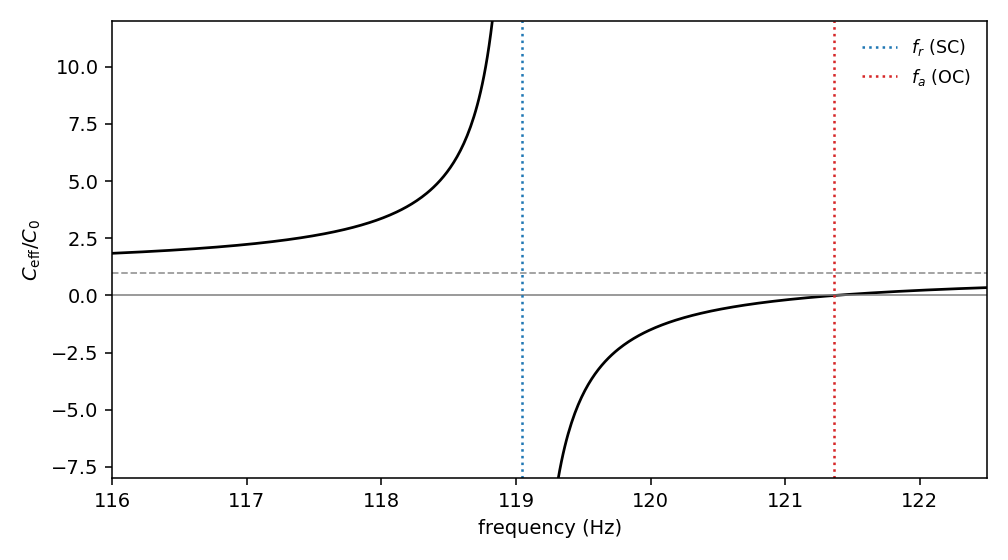
\includegraphics[width=0.92\linewidth]{piezo_p4_admittance_zoom.png}
\caption{Effective capacitance of the driven free--free $n=0$ model at
$h_1/2h=1/12$, $C_0=9.99\,\mathrm{\mu F}$. The pole is the short-circuit
root $f_r=119.046\,\mathrm{Hz}$; the zero is the open-circuit root
$f_a=119.379\,\mathrm{Hz}$.}
\label{fig:Y}
\end{figure}

\section{Discussion}\label{sec:disc}
The numerical inverse never failed. Every round-trip recovered the true
constant to nine figures. What failed, under short-circuit flexure, is
identifiability of $e_{31}$, and it failed for a reason that is in Duan,
Quek and Wang's Fig.~3 and in Green's identity, not in the root search.
Treating that failure as a finding, rather than as a defect to be tuned
away, is what makes the open-circuit $n=0$ result a result: it is the
smallest change of electrical and mechanical boundary conditions that
puts $e_{31}$ on a frequency.

Limits, so they are not rediscovered as objections. The open-circuit
model is leading-order linear potential; the short-circuit $6\times6$
retains the interior potential. Their coupling corrections differ by two
orders of magnitude on the first $n=0$ mode ($0.28\%$ versus $0.0007\%$),
so comparing them as $f_a$ and $f_r$ is consistent at the precision of
\eqref{eq:keff}. This was checked, not only argued from magnitude:
enriching the open-circuit potential with the same interior potential
used by the short-circuit $6\times6$ raises the free--free $n=0$
open-circuit root by $7\times10^{-6}$ relative at $h_1/2h=1/12$, which
is exactly the short-circuit interior stiffening -- under the consistent
projection the two stiffenings simply add, because the uniform bus field
and the interior field are orthogonal in the enthalpy -- so the
leading-order model already used throughout is adequate here. Circumferential orders $n\neq0$ carry no net charge on a
continuous electrode and do not split; three-dimensional finite elements
confirm this at $n=1$--$4$ to $10^{-10}$. Clamped--clamped open-circuit
does not split at this order. Clamped--free $n=0$ open-circuit does,
at nearly the free--free split; free--clamped $n=0$ open-circuit
splits far less, because only the inner hole is free. In-plane piezoelectric coupling, a
monolithic ring, and simultaneous multi-parameter recovery are not
claimed. No laboratory specimen is reported here. Were one measured, the
free--free $n=0$ resonance/antiresonance pair of Table~\ref{tab:inv}
is the observable; the $0.01\%$ column of that table characterizes
inverse conditioning, not a laboratory accuracy target
(Fig.~\ref{fig:noisefloor}).

The elastic ring of McCune and Stutts \cite{mccune2026ring} is the
mechanical baseline this construction sits on. The present frequencies
do not re-score Vogel, Narita, or Irie; they score a piezoelectric table
and an open-circuit splitting that that elastic paper did not contain.

The solver implementing the $6\times6$ and the rank-1 $4\times4$, and
the scripts that produced every table here, are in the public tree
accompanying McCune and Stutts \cite{mccune2026ring}.

\section{Conclusions}\label{sec:conc}
A layered piezoelectric annulus has a short-circuit $6\times6$ that
recovers Duan, Quek and Wang's Table~4 at $27/27$, worst relative error
$-0.049\%$, and a free--free open-circuit $4\times4$ whose first $n=0$
root lies $0.280\%$, $0.405\%$, and $0.601\%$ above the elastic bilayer
at $h_1/2h=1/12$, $1/8$, and $1/5$. Piezoelectric finite elements at all
three ratios reproduce that split against both-faces short-circuit to
within $0.2\%$ of its value, once the bus charge is taken as the
variable conjugate to the bus voltage. Clamped--free open-circuit on the
same mesh reproduces its closed-form $+0.262\%$ split to within
$1.1\%$. Three-dimensional coupled-field elements extend the check
to $n=1$--$4$: open circuit equals short circuit there, and the
short-circuit interior-potential stiffening is reproduced to within
$1.2\%$. Host $E$ is recoverable from one short-circuit
clamped--clamped frequency at $0.025\%$ for $0.01\%$ frequency
precision, and from free--free elastic or open-circuit flexure at the
same $0.025\%$; $e_{31}$ from the clamped--clamped short-circuit
observable is not ($889\%$). The same
$e_{31}$ is recoverable from the free--free axisymmetric open-circuit
frequency at $2.13\%$, $1.48\%$, and $1.00\%$ as the layer thickens,
assuming $E$ known exactly; short-circuit at the same three ratios
remains $889\%$, $294\%$, and $88\%$. Recovering $E$ and $e_{31}$ in
sequence, as an actual measurement would, compounds the $h_1/2h=1/12$
open-circuit figure to $3.01\%$ -- still two orders of magnitude better
than the short-circuit route. The driven admittance
of the open-circuit model has its pole and zero at those two
frequencies at all three Table~4 ratios, with $k_{\mathrm{eff}}=0.075$,
$0.090$, and $0.109$. That
pair, not a short-circuit flexural list, is the identifying observable
for $e_{31}$. A clamped-inner, free-outer ring is a second channel of
the same class ($+0.262\%$ closed-form, reproduced by finite elements
to $1.1\%$, $2.28\%$ of $e_{31}$ at $0.01\%$ frequency); the swapped
pair is not.

\section*{Data and code availability}
The solver implementing the operators of this paper, the scripts that
produced every number and table here, and the finite-element decks with
their text outputs extend the public tree accompanying
\cite{mccune2026ring}.

\section*{Funding}
This research did not receive any specific grant from funding agencies in the
public, commercial, or not-for-profit sectors.

\section*{Acknowledgments}
The computation for this work was performed on The Mill HPC cluster at
Missouri University of Science and Technology \cite{mill2024}. GPU resources
were not used.

\section*{CRediT authorship contribution statement}
\textbf{Garrek McCune:} Conceptualization, Methodology, Software, Validation,
Formal analysis, Investigation, Writing -- original draft, Writing -- review \&
editing, Visualization. \textbf{Daniel Stutts:} Conceptualization,
Supervision.

\section*{Declaration of generative AI and AI-assisted technologies}
During the preparation of this work, the authors used generative AI tools to
assist with manuscript and code organization, drafting, editing, and
formatting. After using these tools, the authors reviewed and edited the
content as needed and take full responsibility for the content of this
publication.
\normalsize

\begin{thebibliography}{99}\small
\setlength{\itemsep}{0pt}
\setlength{\parsep}{0pt}
\bibitem{seok1} J. Seok, H.F. Tiersten, ``Free vibrations of annular sector
cantilever plates. Part 1: out-of-plane motion,'' J. Sound Vib. 271 (2004)
757--772. \url{https://doi.org/10.1016/S0022-460X(03)00414-0}.
\bibitem{seok2} J. Seok, H.F. Tiersten, ``Free vibrations of annular sector
cantilever plates. Part 2: in-plane motion,'' J. Sound Vib. 271 (2004)
773--787. \url{https://doi.org/10.1016/S0022-460X(03)00415-2}.
\bibitem{seok3} J. Seok, H.F. Tiersten, H.A. Scarton, ``Free vibrations of
rectangular cantilever plates. Part 1: out-of-plane motion,'' J. Sound
Vib. 271 (2004) 131--146. \url{https://doi.org/10.1016/S0022-460X(03)00365-1}.
\bibitem{seok4} J. Seok, H.F. Tiersten, H.A. Scarton, ``Free vibrations of
rectangular cantilever plates. Part 2: in-plane motion,'' J. Sound Vib.
271 (2004) 147--158. \url{https://doi.org/10.1016/S0022-460X(03)00366-3}.
\bibitem{duan2005} W.H. Duan, S.T. Quek, Q. Wang, ``Free vibration analysis
of piezoelectric coupled thin and thick annular plate,'' J. Sound Vib. 281
(2005) 119--139. \url{https://doi.org/10.1016/j.jsv.2004.01.005}.
\bibitem{liu2002} X. Liu, Q. Wang, S.T. Quek, ``Analytical solution for free
vibration of piezoelectric coupled moderately thick circular plates,''
Int. J. Solids Struct. 39 (2002) 2129--2151.
\url{https://doi.org/10.1016/S0020-7683(02)00079-3}.
\bibitem{ieee176} IEEE, \emph{IEEE Standard on Piezoelectricity}, ANSI/IEEE
Std 176-1987, IEEE, New York (1988).
\bibitem{hosseini2011} Sh. Hosseini-Hashemi, M. Kalbasi, H. Rokni Damavandi
Taher, ``Free vibration analysis of piezoelectric coupled annular plates
with variable thickness,'' Appl. Math. Model. 35 (2011) 3527--3540.
\url{https://doi.org/10.1016/j.apm.2011.01.003}.
\bibitem{parashar2013} S.K. Parashar, ``Modeling and analysis of
shear-induced flexural vibrations of annular piezoceramic actuators,''
J. Intell. Mater. Syst. Struct. 24 (2013).
\url{https://doi.org/10.1177/1045389X13478273}.
\bibitem{mccune2026annular} G. McCune, D. Stutts, ``Exact wave-function
solution and spurious-mode discrimination for completely free annular sector
plates,'' submitted (2026).
\bibitem{mccune2026rect} G. McCune, D. Stutts, ``Exact wave-function solution
of completely free rectangular plates: four-corner Kirchhoff jump and mode
screening,'' submitted (2026).
\bibitem{mccune2026ring} G. McCune, D. Stutts, ``Exact radial-determinant
frequencies of annular and circular plates: the closed-ring and solid-disk
limits of the sector wave-function method,'' submitted (2026).
\bibitem{boeringa2026} Z.L. Boeringa, G.H. McCune, D.S. Stutts, ``Canonical
validation and model discrimination in a linearly tapered non-uniform rod,''
unpublished manuscript (2026).
\bibitem{ansys} ANSYS, Inc., \emph{ANSYS Mechanical APDL}, Release 2025 R1,
ANSYS, Inc., Canonsburg, PA, USA (2025). Used for finite-element validation
only.
\bibitem{mill2024} Missouri University of Science and Technology, ``The Mill
HPC Cluster,'' \emph{The Mill} (2024), Article 1.
\url{https://scholarsmine.mst.edu/the-mill/1},
\url{https://doi.org/10.71674/PH64-N397}.
\end{thebibliography}
\end{document}
